% ============================================================
%  CHAPTER 3: REQUIREMENTS ANALYSIS AND SPECIFICATION
% ============================================================

\chapter{REQUIREMENTS ANALYSIS AND SPECIFICATION}
\label{chap:requirements}

\section{Functional Requirements Specification}
\label{sec:functional_requirements}

The functional requirements define the explicit operational capabilities of the QuantumSafe VPN system:
\begin{enumerate}[label=FR-\arabic*, leftmargin=1.8cm]
    \item Post-Quantum Handshake Negotiation: The client and gateway must execute an authenticated key exchange using ML-DSA-65 (FIPS 204) and ML-KEM-1024 (FIPS 203) without exposing sensitive keys.
    \item Dynamic Virtual IP Leasing: The server must lease a private IPv4 address from the `10.8.0.0/24` subnet upon successful handshake authentication.
    \item Full Tunnel IP Encapsulation: The Android \texttt{VpnService} must capture all outbound device IPv4 traffic (\texttt{0.0.0.0/0}) and route it into the encrypted tunnel.
    \item Symmetric Encryption with Replay Protection: All payload frames must be encrypted with hardware-accelerated AES-256-GCM authenticated encryption utilizing a 64-bit monotonically increasing sequence counter.
    \item DNS Leak Prevention: Outbound DNS requests must be forcefully bound to verified recursive resolvers (`1.1.1.1` and `8.8.8.8`) through the encrypted tunnel.
    \item Connection Management and Recovery: The application must support manual connect/disconnect toggling and automatic graceful resource cleanup upon network drops.
\end{enumerate}

\section{Non-Functional Requirements Specification}
\label{sec:non_functional_requirements}

The non-functional requirements enforce performance, security, and mobile usability constraints:
\begin{enumerate}[label=NFR-\arabic*, leftmargin=1.8cm]
    \item Post-Quantum Security Level: The system must deliver NIST Security Level 5 ($>256$ bits of classical and quantum hardness).
    \item Handshake Latency: Handshake completion over 4G/5G/Wi-Fi links must terminate in under 150\,ms under nominal conditions.
    \item Memory Footprint: The Android background service must maintain resident memory consumption below 60\,MB.
    \item Battery Efficiency: Zero active CPU spinning during idle connection states; non-blocking asynchronous socket polling.
\end{enumerate}

\section{Use Case Analysis}
\label{sec:use_case_analysis}

Figure~\ref{fig:use_case_diagram} depicts the system use-case diagram illustrating interactions between the Mobile User, Cryptographic Subsystem, and Linux VPN Gateway.

\begin{figure}[!t]
  \centering
  \begin{tikzpicture}[
    actor/.style={draw, thick, fill=blue!10, rounded corners=3pt, minimum width=2.4cm, minimum height=1.0cm, align=center, font=\bfseries\small},
    usecase/.style={draw=vpnblue, thick, fill=white, rounded corners=12pt, minimum width=3.4cm, minimum height=0.9cm, align=center, font=\small},
    systembox/.style={draw=darkcharcoal, dashed, thick, rounded corners=8pt, fill=gray!5, inner sep=12pt}
  ]
    \node[actor] (user) at (-4.5, 0) {Mobile User};
    \node[actor] (gateway) at (4.5, 0) {VPN Gateway};

    \node[usecase] (uc1) at (0, 2.2) {UC-01: Initiate PQC Connection};
    \node[usecase] (uc2) at (0, 0.7) {UC-02: Authenticate Identity};
    \node[usecase] (uc3) at (0, -0.8) {UC-03: Route Encrypted Traffic};
    \node[usecase] (uc4) at (0, -2.3) {UC-04: Terminate Session};

    \begin{scope}[on background layer]
      \node[systembox, fit=(uc1) (uc2) (uc3) (uc4), label=above:{\bfseries\small QuantumSafe VPN System Boundary}] {};
    \end{scope}

    \draw[thick, ->] (user) -- (uc1);
    \draw[thick, ->] (user) -- (uc2);
    \draw[thick, ->] (user) -- (uc3);
    \draw[thick, ->] (user) -- (uc4);
    \draw[thick, ->] (gateway) -- (uc1);
    \draw[thick, ->] (gateway) -- (uc2);
    \draw[thick, ->] (gateway) -- (uc3);
    \draw[thick, ->] (gateway) -- (uc4);
  \end{tikzpicture}
  \caption{Use Case Diagram of QuantumSafe VPN System.}
  \label{fig:use_case_diagram}
\end{figure}

\section{Trust Boundaries and Threat Modeling}
\label{sec:trust_boundaries}

Figure~\ref{fig:threat_model_concept} illustrates the architectural trust boundaries dividing the trusted mobile execution perimeter from the untrusted transit carrier network and the trusted security gateway.

\begin{figure}[!b]
  \centering
  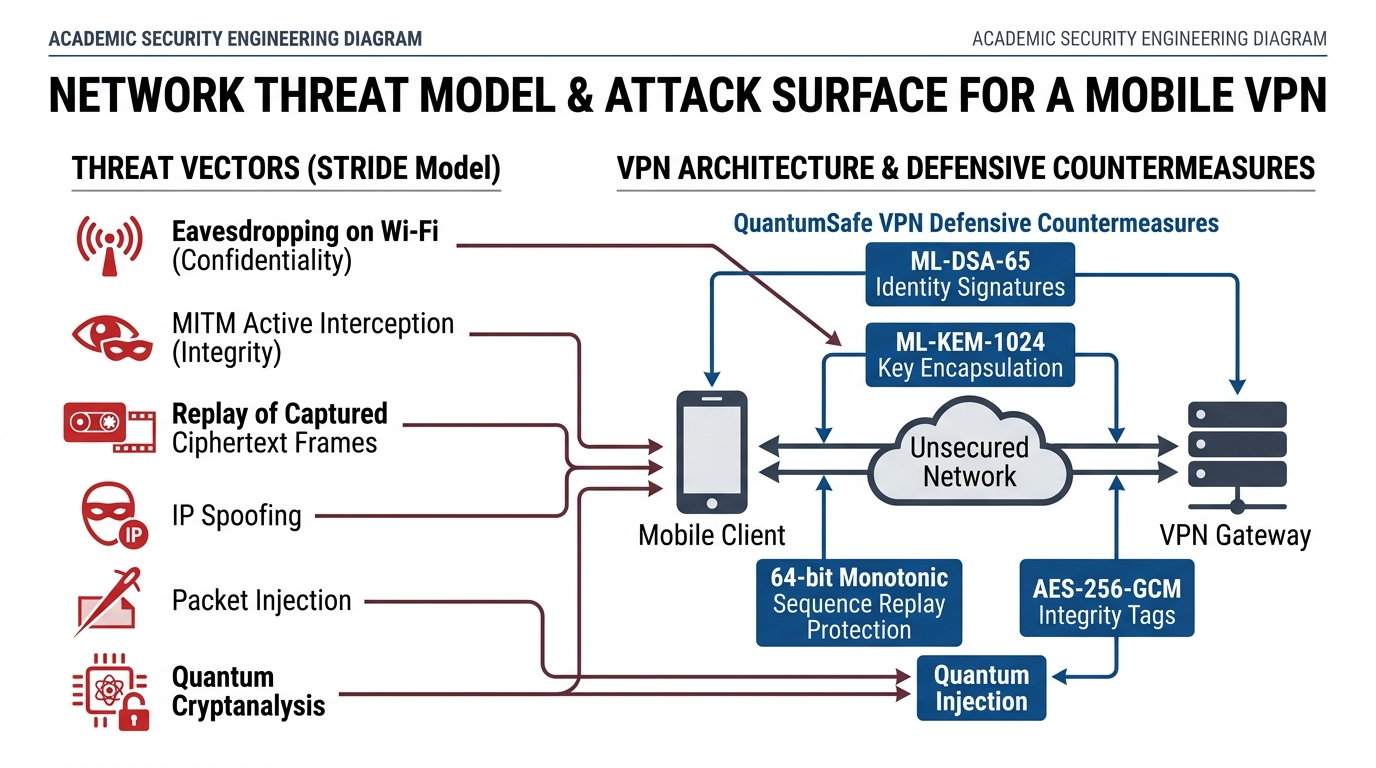
\includegraphics[width=0.88\linewidth,height=0.30\textheight,keepaspectratio]{figures/threat_model_concept.jpg}
  \caption{Architectural Trust Boundaries and Network Threat Vectors.}
  \label{fig:threat_model_concept}
\end{figure}

\section{Requirement Traceability Matrix}
\label{sec:rtm}

Table~\ref{tab:rtm_matrix} provides the Requirement Traceability Matrix (RTM) linking requirements to design and verification modules.

\begin{table}[htbp]
  \centering
  \footnotesize
  \setlength{\tabcolsep}{3pt}
  \caption{Requirement Traceability Matrix (RTM).}
  \label{tab:rtm_matrix}
  \begin{tabularx}{\linewidth}{@{}p{1.4cm}p{3.0cm}p{3.5cm}Yp{1.9cm}@{}}
    \toprule
    \textbf{Req ID} & \textbf{Requirement Name} & \textbf{Design Element} & \textbf{Implementation} & \textbf{Test Case} \\
    \midrule
    FR-01 & PQC Handshake & Stage 1--4 Handshake FSM & \texttt{PqcEngine.kt} & TC-SEC-01 \\
    FR-02 & Dynamic IP Lease & IP Pool Subsystem & \texttt{ip\_pool.py} & TC-INT-02 \\
    FR-03 & Full Tunnel Routing & VpnService TUN Capture & \texttt{QuantumSafe}\allowbreak\texttt{VpnService} & TC-VPN-01 \\
    FR-04 & AES-256-GCM AEAD & Frame Crypto Engine & \texttt{classical.py} & TC-SEC-03 \\
    FR-05 & Anti-Replay Guard & 64-bit Sequence Counter & \texttt{PqcEngine.kt} & TC-SEC-04 \\
    FR-06 & DNS Leak Defense & Explicit Resolver Binding & \texttt{VpnService.}\allowbreak\texttt{Builder} & TC-NET-01 \\
    \bottomrule
  \end{tabularx}
\end{table}
